\subsection{Video life cycle}
\begin{frame}[fragile]	
	\frametitle{Video life cycle}
	\begin{figure}[!t]
		\centering
		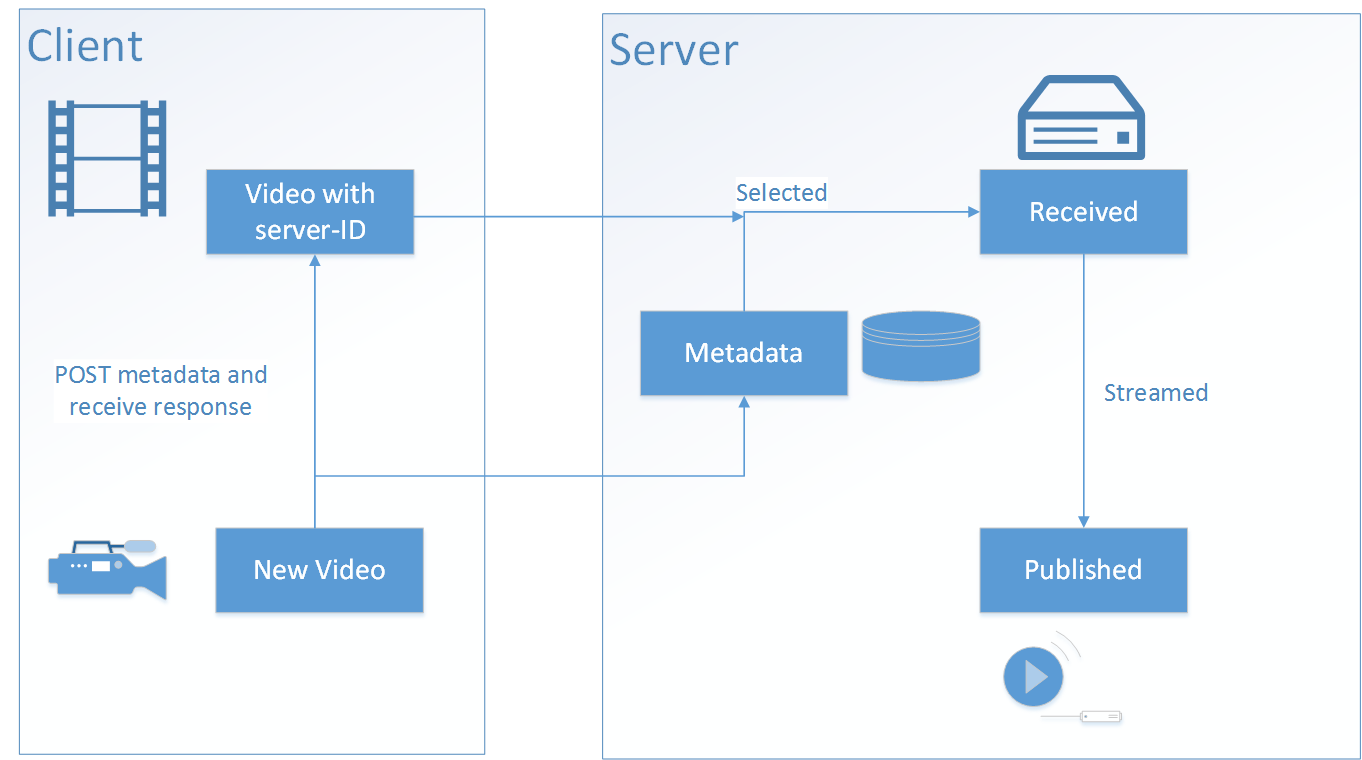
\includegraphics[width=\textwidth,height=\textheight,keepaspectratio]{video_states.png}
		\label{fig:states}
	\end{figure}
\end{frame}
\subsection{Selection algorithm}
\begin{frame}	
	\frametitle{Selection algorithm}
	% TODO
	\tiny
The \texttt{VideoRating} class provides static functionality to rank videos by certain criteria. This is done by providing
a set of data that depends on the video duration. In the current implementation, you input video metadata and the
rating system will transform these values, which are defined from 0 to infinity, down to [0, 1] using a sigmoid function,
then account for the duration of the video. This is done because shorter videos should get heavier penalties for
having the same amount or more shaking and tilting as a longer duration video. The function is applied separately to
shaking and tilting, and afterwards they are combined into a score using a kernel with weights. The final score is
then multiplied by 100, so that the final range is [0, 100]. This process happens before video metadata is stored
in the database, as the video itself never changes, and helps the video upload selection process later on.

When selecting a video for upload, given a client, the server will consider all pending videos that client,
then for each event of a video (should be just one) check if the client has any pending videos that
are top candidates for that events stream. This is done by asking for the subset of videos which start after
the event timestamp, and then sorting by video rank. This ensures that the video closest to the events
timestamp gets selected, so that its possible to maintain a stream of videos sequentially which are determined
to be of good quality. It also unfortunately means that there can be gaps between videos, and that with not
enough videos low quality will be selected. After receiving a selected video, the server immediately sets the
new event timestamp, so even if a new video appears that is of much higher quality, or is more directly
sequential to the last one, the server will end up using the ``guaranteed'' video it just received. This could
be alleviated somewhat by having a potential stream running with a bigger delay from the main event, and then
doing more intelligent rebuilding of the stream.
\end{frame}